\documentclass[11pt]{article}
\usepackage[margin=1in]{geometry}
\usepackage[T1]{fontenc}
\usepackage{lmodern}
\usepackage{amsmath}
\usepackage{booktabs}
\usepackage{graphicx}
\usepackage{subcaption}
\usepackage{pgfplots}
\usepgfplotslibrary{fillbetween}
\pgfplotsset{compat=1.18}
\usepackage{xurl}
\usepackage[hidelinks]{hyperref}
\hypersetup{pdftitle={essentialism: An On-Chain Generative Work That Forgets Two Photographs}, pdfauthor={Benjamin Meadows}, pdfkeywords={generative art, on-chain art, Tezos, memory, forgetting, digital preservation}}
\usepackage{natbib}
\usepackage{xcolor}
\setlength{\parskip}{0.35em}

\definecolor{inkblue}{HTML}{36597D}
\definecolor{inkpink}{HTML}{DD68A4}
\definecolor{ember}{HTML}{E0521B}

\title{\texttt{essentialism}: An On-Chain Generative Work\\That Forgets Two Photographs}
\author{Benjamin Meadows\\Independent Artist and Researcher\\\texttt{ben@benjaminmeadows.com}}
\date{October 2026}

\begin{document}
\maketitle

\begin{abstract}
\texttt{essentialism} is a generative artwork of 44 editions whose program is stored on the Tezos blockchain. It carries two of my photographs inside its code as $28\times38$ grids of 16 gray levels. Each edition samples its grid at a weight fixed by the edition number, 100\% at edition 1 falling linearly to 12\% at edition 44, mixed with value noise whose weight rises as the photograph's falls, and each token states that weight in its trait line as its ``memory''. The ledger keeps the program, and in its block history every superseded version of it; the editions are where the work forgets. Over 1{,}000 seeds and all 44 editions (44{,}000 renders) I measured how strongly each photograph still shows in the generator's internal darkness field and in the ink of the drawn dots. The field keeps a median correlation of at least 0.94 with the photograph through edition 21 and loses 0.43 (tree) and 0.44 (sky) of it between editions 34 and 44: a signal weight that falls linearly against a rising noise weight gives a correlation that holds and then drops. A closed form with two measured variances reproduces the field curve to within 0.010 for one photograph and 0.021 for the other. Counting every render, the dots' ink keeps a median rank correlation of 0.82 with the tree photograph at edition 1 and 0.14 at edition 44, against medians between 0.00 and 0.104 for a counterfactual null in which the other photograph drives a re-render of the same seed. The decline is orderly in the medians, not token by token, and the memory percentage printed on each token is above the median drawn correlation through edition 11 and below it from edition 12, with one exception. Nine editions are minted; the latest states a memory of 84\%, and renders at its edition number have a median drawn correlation of 0.79 (tree) or 0.81 (sky). The ledger also kept something I would have chosen to forget: the first published version of the code claimed an algorithm that was not mine. Separately, the platform's image of a minted token could not be reproduced from the seed data it stores on chain. The generator, measurement scripts, data and this paper's source rebuild from one command.
\end{abstract}

\section{The work}

\texttt{essentialism} \citep{essentialism2026} was published on 31 July 2026 as generator 407 on bootloader \citep{bootloader}, a platform on Tezos \citep{goodman2014} that stores a generative program in a contract's storage and renders each token in the browser from that program and a per-token seed. Generators that live entirely on a ledger go back at least to Larva Labs' Autoglyphs, whose drawing code sits in its Ethereum contract \citep{larvalabs2019}. The edition is 44 tokens at 8 tez. Each token is a $750\times1000$ SVG: columns of dots dropped down a sheet of paper, colored from a small library of inks.

The column structure is not mine. In November 2022 I worked through Andy Haskell's tutorial on converting images to mosaics in p5.js \citep{haskell2022}, randomized the dot size, pointed it at my own photographs, and saved nine test outputs under the name Essentialism without releasing them. In the tutorial's version, and in mine, each dot asks a photograph for its color. The bootloader runtime allows no external files, so the on-chain program cannot load a photograph, and in July 2026 I had to decide what the dots would ask instead.

They ask two photographs that were reduced until they fit in the code. ``Blue Tree'' \citep{bluetree2023} is a photograph of a tree that was removed after a storm in December 2023, three months after I minted the image on Ethereum, so the picture has outlived its subject. ``Natural Gradient'' \citep{naturalgradient2023} is an unedited sky whose full-resolution file sits on Arweave \citep{williams2019}. Both originals are minted; how long their image files stay retrievable depends on the services that hold them. The work embeds a coarse copy of each and lets that copy fade across the edition: edition 1 samples its photograph at full strength, and edition 44 at 12\%. The dots take their ink from what is left. Figure~\ref{fig:strip} shows one seed at four editions.

\begin{figure}[t]
  \centering
  \begin{subfigure}{0.24\textwidth}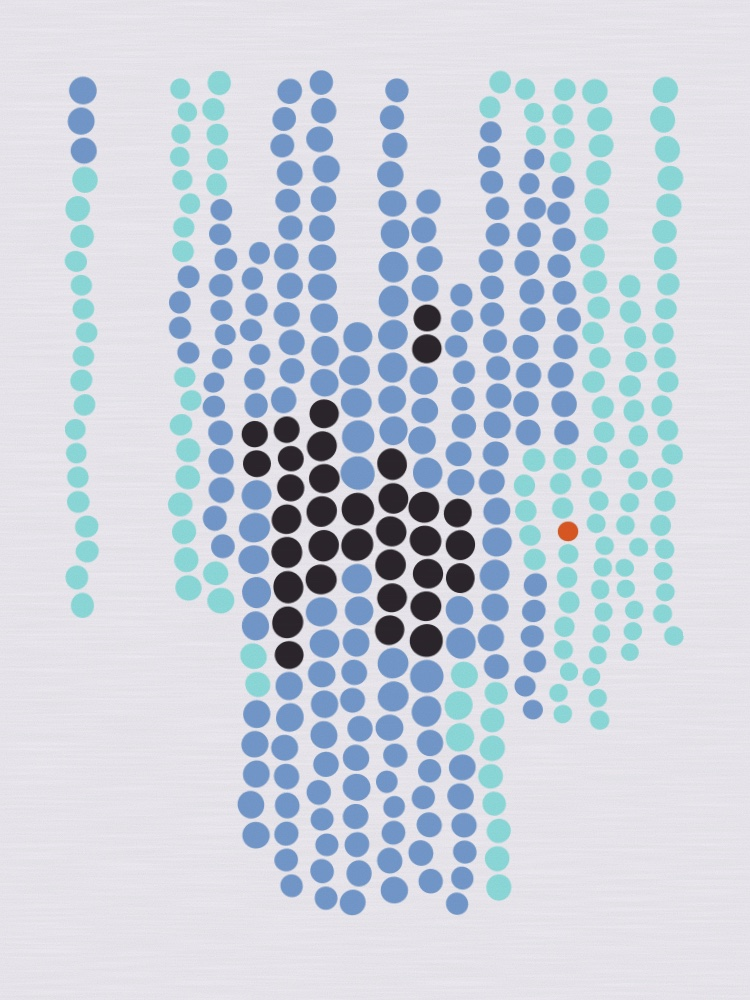
\includegraphics[width=\linewidth]{figures/strip-ed01.jpg}\caption*{ed.\ 1, memory 100\%}\end{subfigure}\hfill
  \begin{subfigure}{0.24\textwidth}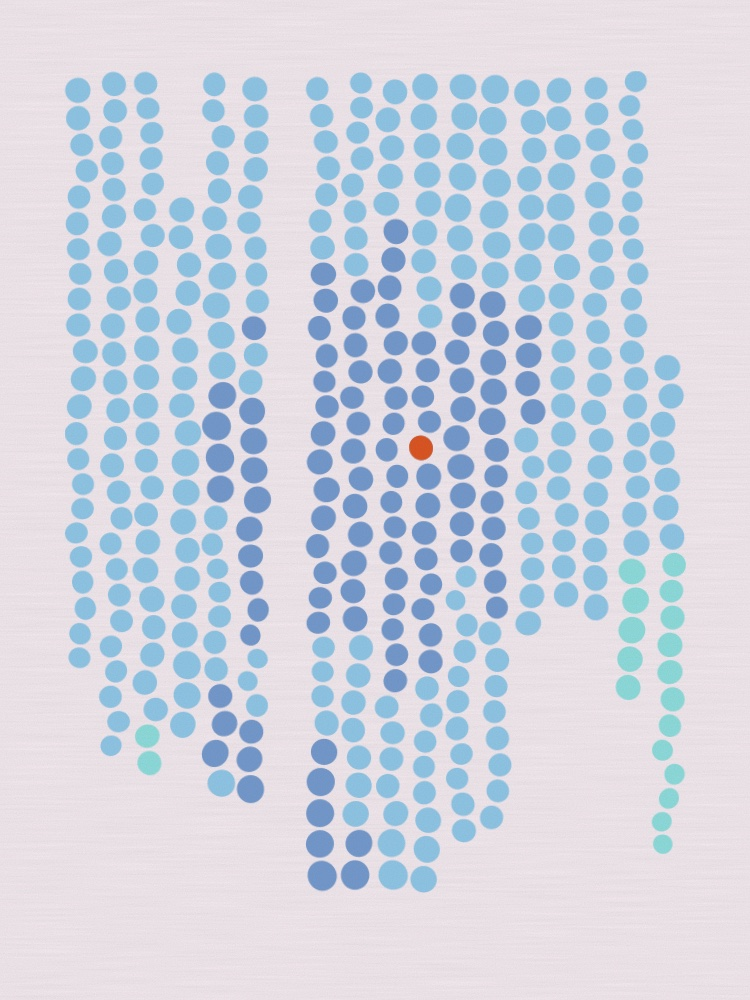
\includegraphics[width=\linewidth]{figures/strip-ed15.jpg}\caption*{ed.\ 15, memory 71\%}\end{subfigure}\hfill
  \begin{subfigure}{0.24\textwidth}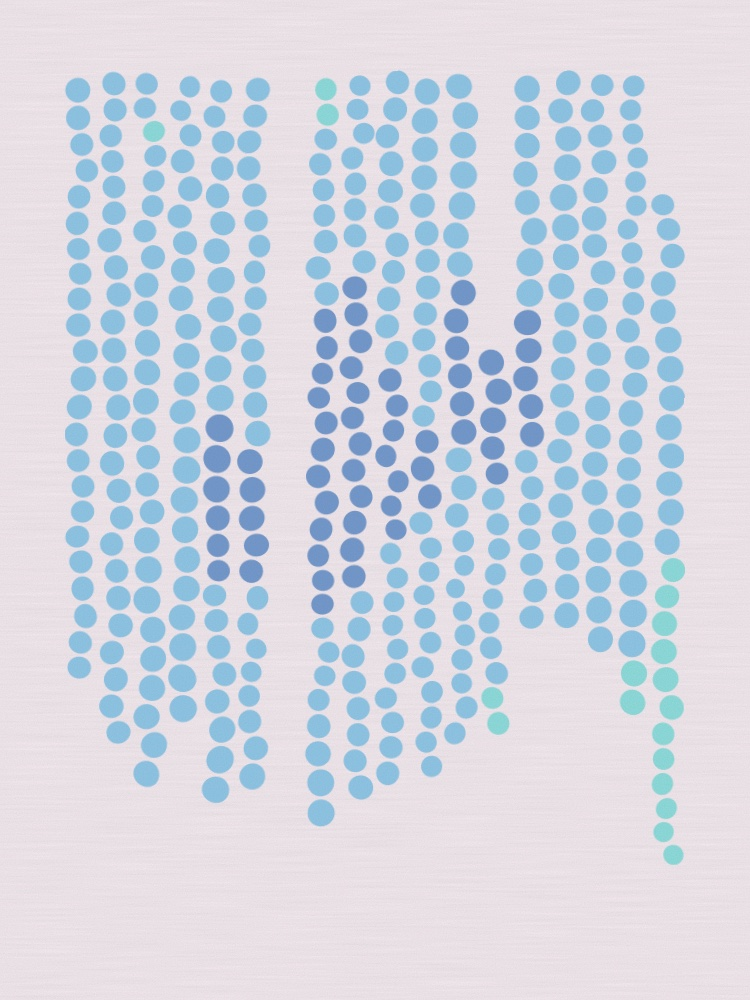
\includegraphics[width=\linewidth]{figures/strip-ed30.jpg}\caption*{ed.\ 30, memory 41\%}\end{subfigure}\hfill
  \begin{subfigure}{0.24\textwidth}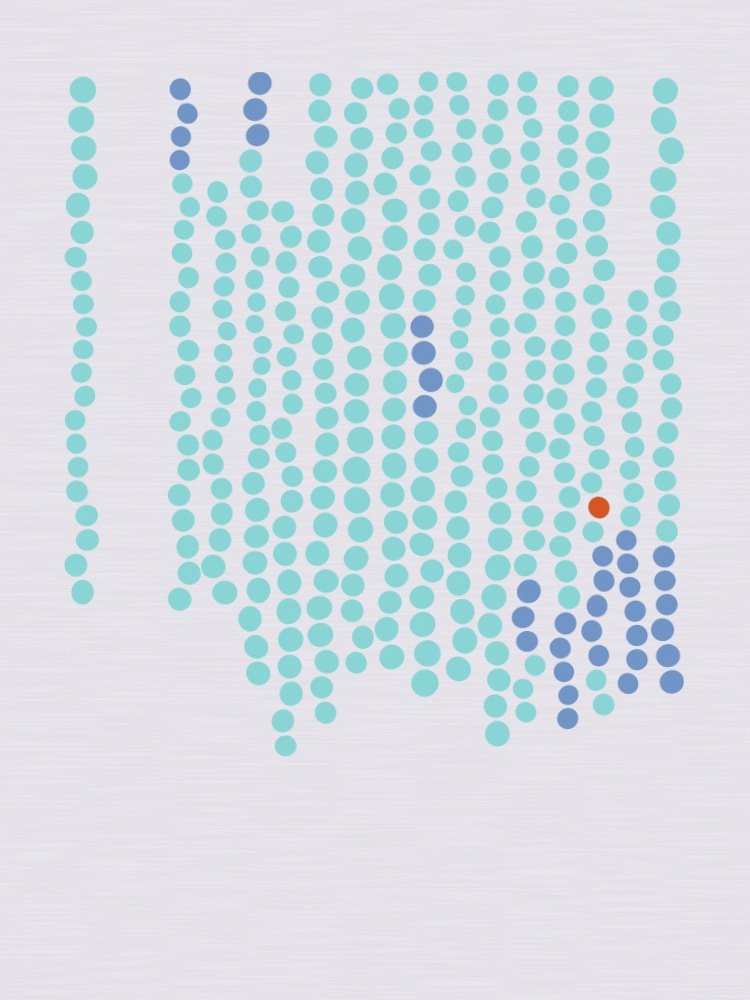
\includegraphics[width=\linewidth]{figures/strip-ed44.jpg}\caption*{ed.\ 44, memory 12\%}\end{subfigure}
  \caption{One seed (1391882777, edition 1's stored entropy reduced modulo $2^{32}$) drawn at four edition numbers by the on-chain generator, version 6. Traits: field density, two inks, source ``blue tree'', one ember. The dark mass at edition 1 is the trunk and crown of the tree. This is not the platform's image of edition 1, which comes from a seed I could not derive (Section~\ref{sec:ledger}). Only the memory factor changes across the row, but because the dot sizes and run lengths depend on the memory field, the composition shifts as well. Rendered by \texttt{repro/figures.mjs}, rasterized with Inkscape 1.4.4.}
  \label{fig:strip}
\end{figure}

Every token states a ``memory'' percentage in its trait line. Before writing this paper I had not checked how much of a photograph that percentage leaves in the drawing.

\section{Two ways of keeping}
\label{sec:context}

In relearning experiments, most of what is lost is lost early. Ebbinghaus measured his own relearning savings for nonsense syllables at intervals from twenty minutes to a month and found the steepest decline in the first hour \citep{ebbinghaus1885}; a replication with the same method reproduced the curve \citep{murre2015}, and in three experiments and a reanalysis of Ebbinghaus's data, forgetting was best described by a power function of time, whose rate of loss falls with time \citep{wixted1991}. Forgetting in this literature is a property of the rememberer.

Digital storage is often assumed to remove forgetting, and it does not. Bits decay and the systems holding them fail \citep{rosenthal2010}; one in five science, technology and medicine articles suffers from reference rot, and seven in ten of those that cite web resources do \citep{klein2014}, and half of the URLs in United States Supreme Court opinions no longer pointed to the cited material when Zittrain, Albert and Lessig checked \citep{zittrain2014}. Chun describes digital media as an ``enduring ephemeral'': always available in principle, regenerated constantly in practice, and liable to vanish \citep{chun2008}. Ernst argues that the digital archive is an operation rather than a store \citep{ernst2013}, and Kirschenbaum shows how much of a file's history persists physically even after it is ``deleted'' \citep{kirschenbaum2008}. Rinehart and Ippolito argue that the vulnerability of new media art, whose software and hardware change faster than institutions' preservation methods, illustrates a larger crisis for social memory \citep{rinehart2014}.

A blockchain promises the opposite for the bytes written to it. A ledger replicated across independent nodes and extended only by appending blocks \citep{nakamoto2008,wood2014,goodman2014} offers no operation that removes a past state; a contract can overwrite the current value of a key, but every earlier value stays in the block that wrote it, and archive nodes and indexers continue to serve it. Not every node does: in rolling mode a node keeps only recent blocks, and in full mode it keeps every block, including the transactions that carried each version's code, but prunes old state and receipts \citep{octezhistory}. The current value of a key is part of the live state every node holds; a superseded value survives because someone chooses to keep the history. The cost is paid once, per byte: on Tezos, 250 mutez (0.00025 tez) for every byte added to a contract's storage. Superseded values are not charged again. For larger files, content addressing guarantees that a file is the one named, though not that anyone still serves it \citep{benet2014}, and Arweave's storage endowment is designed to pay for continued availability \citep{williams2019}. This permanence collides with law that treats forgetting as a right. Article 17 of the GDPR gives a data subject the right to erasure \citep{gdpr2016}; two years earlier, under the Data Protection Directive it replaced, the Court of Justice had required a search engine to delist links to outdated information about a person in \emph{Google Spain} \citep{googlespain2014}. Finck sets out why an append-only ledger cannot comply in any straightforward way \citep{finck2018}. Mayer-Sch{\"o}nberger argues for building expiry into information systems by default \citep{mayerschonberger2009}, and Bannon for treating forgetting as a design feature rather than a defect \citep{bannon2006}. Borges's Funes, who cannot forget anything, also cannot think, because thinking requires discarding differences \citep{borges1944}.

Artists have staged loss as a process for decades. Lucier rerecorded his voice in a room until the room's resonances replaced the words \citep{lucier1969}; Basinski played decaying tape loops until the oxide shed from them \citep{basinski2002}; Metzger's manifesto proposed works whose making was their destruction \citep{metzger1959}. Opa{\l}ka's count is the nearest to a fading sequence: from 1972 each canvas was painted on a ground about 1\% whiter than the one before, so the series whitens as it goes on \citep{opalka1965}. Simon's \emph{Every Icon} runs a process toward an end no viewer will see \citep{simon1997}. On ledgers, Friend's \emph{Lifeforms} are tokens that die unless their holder gives them away within 90 days \citep{friend2021}, and some editions already key the work to mint order: in Reas's \emph{923 EMPTY ROOMS} the mint number selects the composition \citep{reas2023}, and in Gerrard's \emph{World Flag} release order follows each country's greenhouse-gas ranking \citep{gerrard2023}. Weaker later copies are old in print: a drypoint plate's burr wears away so quickly that only about a dozen good impressions can be taken \citep{met2003drypoint}, and Burn's \emph{Xerox Book} is a hundred successive photocopies of a blank sheet, bound in order \citep{burn1968}. On a ledger nothing wears, and I have not found an on-chain edition that schedules such a decline. Lucier's tape, Basinski's loops and Metzger's objects lose their material. \texttt{essentialism} cannot: until the generator is updated again, its current program, and with it both grids, is part of the ledger's live state, held by every node. The only thing the work can vary is the edition counter, so that is where the forgetting goes. Each token's memory weight is fixed at mint and never changes afterwards; the schedule runs in the order the edition is minted, and earlier tokens keep what they were given. Barthes located a photograph's force in its ``that-has-been'' \citep{barthes1981}, a claim that the thing was there. Here the photograph stays in the code, and what the edition number lowers is how much of it the drawing shows.

\section{Construction}
\label{sec:construction}

The generator is 10{,}098 bytes of JavaScript (generator version 6, SHA-256 \texttt{33d85a12\ldots c248}; the full digest is in Section~\ref{sec:repro}). It is stored URI-encoded, 15{,}560 bytes, and runs in bootloader's SVG-JS runtime, which provides an SVG root, a seeded generator \texttt{rnd()} built from splitmix64 \citep{steele2014} feeding sfc32 \citep{practrand}, and the token's \texttt{iterationNumber}. Line numbers below refer to the stored code.

\paragraph{The grids.} Each photograph was converted to grayscale, center-cropped to the grid's $28\times38$ aspect (close to the sheet's $3\times4$), autocontrasted with a 1\% cutoff, resampled to $28\times38$ cells, and quantized to 16 levels, written one hexadecimal character per cell: 1{,}064 bytes per photograph, carrying at most 532 bytes of information. Both strings are literals in the code (lines 25 and 26). Storing the two cost $2{,}128 \times 250$ mutez $= 0.532$ tez. Steyerl's poor image gives up resolution to circulate \citep{steyerl2009}; these grids gave it up to fit in contract storage. The grids correlate with each other at $r = 0.10$ over cells. Figure~\ref{fig:grids} shows both.

\begin{figure}[t]
  \centering
  \begin{tikzpicture}
    \begin{axis}[name=tree, width=5.4cm, height=7.2cm, axis equal image, y dir=reverse,
      hide axis, colormap/blackwhite, point meta min=0, point meta max=15, title={\small blue tree}]
      \addplot [matrix plot*, mesh/cols=28, point meta=explicit] table [x=i, y=j, meta=tree, col sep=comma] {data/grids.csv};
    \end{axis}
    \begin{axis}[at={(tree.east)}, anchor=west, xshift=1cm, width=5.4cm, height=7.2cm, axis equal image, y dir=reverse,
      hide axis, colormap/blackwhite, point meta min=0, point meta max=15, title={\small natural gradient}]
      \addplot [matrix plot*, mesh/cols=28, point meta=explicit] table [x=i, y=j, meta=sky, col sep=comma] {data/grids.csv};
    \end{axis}
  \end{tikzpicture}
  \caption{The two photographs as the ledger holds them: $28\times38$ cells, 16 gray levels, read from the generator's string literals by \texttt{repro/field.mjs}. This is the most of either photograph any edition can recall.}
  \label{fig:grids}
\end{figure}

\paragraph{The memory field.} Let $P(x,y)\in[0,1]$ be the bilinear interpolation of the token's grid at canvas position $(x,y)$, where 1 is the lightest level, and let $n(x,y)$ be two octaves of value noise \citep{perlin1985} over a $16\times16$ lattice drawn from the first 256 outputs of \texttt{rnd()} (lines 35 to 42). The generator draws from a darkness field
\begin{equation}
  D(x,y) \;=\; f\,\bigl(1 - P(x,y)\bigr) \;+\; 0.85\,(1-f)\, n\!\left(3.1\tfrac{x}{W} + 5.2,\; 3.1\tfrac{y}{H}\right),
  \label{eq:field}
\end{equation}
with memory factor
\begin{equation}
  f(e) \;=\; \max\!\left(0.12,\; 1 - 0.88\,\frac{\min(e, 44) - 1}{43}\right)
  \label{eq:memory}
\end{equation}
for edition number $e$ (line 69). Over $e = 1,\ldots,44$ the floor never binds: $f$ falls by $0.88/43 \approx 0.0205$ per edition from 1 to exactly 0.12. Platform previews use $f = 1$.

\paragraph{Columns and dots.} The canvas is divided into columns of width $3r_0$, where $r_0$ is a base dot radius drawn per token; the factor 3 and the column-of-dots loop are Haskell's \citep{haskell2022}. Whether a column is drawn, and how far down it runs, depends on a noise value per column and on $D$ at the column's center. Down each column the generator places dots of radius $r = r_0\,(0.72 + 0.56\,n')(0.8 + 0.5\,D)$, so dark regions of the memory field get larger dots and longer runs. Each dot's ink is chosen from $D$ at its center: the token's $k$ inks are sorted from light to dark and indexed by $\lfloor kD \rfloor$; below $D = 0.1$ the dot is usually bone paper color, and above $0.88$ usually carbon. With probability 0.58 a dot repeats the previous dot's ink when $D$ has changed by less than 0.3 since that dot (line 129), which turns per-dot color noise into runs that break where the picture changes. On night paper the ink order is reversed. A static analogue is the column-structured ordered dither of print halftoning \citep{ulichney1987}, with the dither threshold replaced by a field whose photographic weight falls with the edition number.

\paragraph{Inks and traits.} The five inks are colors I had already used in earlier on-chain works and listed in a palette file before this project began: pink and pale blue from ``together'', two blues from ``overhead'', and a pale blue labeled ``mr.\ blue sky'' whose source work I can no longer identify. Bone and carbon come from earlier noise studies, and the single ember dot (\textcolor{ember}{\#e0521b}) from the fourth 2022 test output. Table~\ref{tab:traits} lists the seeded traits with the weights written in the code and their frequencies over 20{,}000 seeds; every observed share is within 1.5 standard errors of its weight. Memory is the only trait not drawn from the seed. Each token writes its traits, including memory as a percentage, into the SVG's \texttt{desc} element (line 153).

\begin{table}[t]
  \centering
  \small
  \begin{tabular}{llrr}
    \toprule
    trait & value & weight in code & observed (20{,}000 seeds) \\
    \midrule
    density & air / field / full & 50 / 38 / 12\% & 49.7 / 38.1 / 12.3\% \\
    inks & 1 / 2 / 3 / 4 & 4 / 56 / 30 / 10\% & 3.8 / 56.2 / 29.9 / 10.1\% \\
    source & blue tree / natural gradient & 87 / 13\% & 86.8 / 13.2\% \\
    paper & night (carbon) & 8\% & 8.1\% \\
    ember & present & 55\% & 54.8\% \\
    memory & edition-determined & Eq.~\eqref{eq:memory} & n/a \\
    \bottomrule
  \end{tabular}
  \caption{Seeded traits. Observed shares from \texttt{repro/census.mjs} at edition 1; the largest deviation is 1.44 standard errors (one ink). The five non-night papers (blush, ivory, rose, fog, overhead blue at 28/22/20/12/10\%) are not reported in the trait line and were not counted.}
  \label{tab:traits}
\end{table}

\section{What the editions remember}
\label{sec:measure}

The trait line asserts a memory percentage, which is $f(e)$ and nothing more. Whether a viewer, or a program, could recover the photograph from a finished edition is a different question, and the answer depends on everything between Eq.~\eqref{eq:field} and the drawn dots. I measured it at two stages.

\paragraph{Method.} For the field, I rebuilt $n$ for each seed from the first 256 draws of its PRNG, evaluated Eq.~\eqref{eq:field} on a $75\times100$ lattice, and computed the Pearson correlation between $D$ and the photograph's darkness $1-P$, for both photographs at every edition (\path{repro/field.mjs}). Neither measure is an information bound. The photograph is never lost from the work: both grids sit in the code, and with the seed's noise any edition's field can be inverted exactly, $1-P = \bigl(D - 0.85(1-f)\,n\bigr)/f$. What the measures track is how strongly the photograph shows in the field and in the drawing. For the drawing, I rendered each (seed, edition) pair with the stored generator, took every dot except the ember, and computed the Spearman rank correlation between the dot's ink darkness (one minus Rec.~601 luma) and the photograph's darkness at the dot's center (\path{repro/measure.mjs}). Centers are taken before the texture filter, which displaces each dot by at most 3 pixels, about a ninth of a grid cell. A token's ink darkness takes at most $k+2$ values ($k$ inks, bone and carbon), so ties alone keep the rank correlation below 1 even at full memory. Night-paper tokens invert the ink order by design, so their correlations are sign-flipped; at edition 1 their median is 0.80, against 0.83 over all 1{,}000 seeds. The measure reads ink only, although dot size, column presence and run length also follow $D$; a second measure below counts those too. In 3{,}291 renders (7.5\%) every dot has the same ink and the rank correlation is undefined. I score these 0, since their ink carries no rank information about the photograph, so every render counts. For tree tokens their share rises from 1.0\% at edition 1 to 13.3\% at edition 42 (12.7\% at edition 44); dropping them instead would raise the edition-44 median from 0.14 to 0.19. Seeds are $1{,}000{,}003 + 7{,}919\,i$ for $i = 1,\ldots,1000$, giving 44{,}000 renders, 872 of each edition from tree tokens and 128 from sky tokens. Because the PRNG stream depends on the seed alone, the 44 renders of one seed share every trait drawn before the dots (all but the ember); the curves pool over seeds, not over editions.

\paragraph{A counterfactual null.} For each (seed, edition) I also render the same program with only the photograph swapped: the source draw still consumes its random number, and every trait except the ember is drawn before the dots, so those traits come out the same; in 600 checked pairs they all matched (the ember is drawn after the dots and can differ) (\texttt{renderSwapped} in \path{repro/runtime.mjs}; the stored code is not modified). Inside the dot loop, dot sizes, run lengths and the random draws follow the other photograph. The dots of that render are correlated with the photograph the real token sampled. This is a replacement control: it shows what the same token would look like if the other photograph drove it, not what a token with no photograph would look like.

\paragraph{A closed form for the field.} If the noise is uncorrelated with the photograph, Eq.~\eqref{eq:field} gives
\begin{equation}
  \rho_{\text{field}}(f) \;\approx\; \frac{f\,\sigma_p}{\sqrt{f^2\sigma_p^2 + 0.85^2(1-f)^2\sigma_n^2}},
  \label{eq:closed}
\end{equation}
where $\sigma_p$ is the standard deviation of the photograph's darkness over the canvas and $\sigma_n$ that of the noise. Measured (\path{repro/sigma.mjs}): $\sigma_p = 0.2515$ for the tree and $0.2601$ for the sky; the median $\sigma_n$ over 1{,}000 seeds is $0.1486$. The photograph and the noise contribute equal spread where $f\sigma_p = 0.85(1-f)\sigma_n$, at $f^\ast = 0.334$ for the tree and $0.327$ for the sky, which Eq.~\eqref{eq:memory} reaches at edition 33.5 and 33.9. At $f^\ast$ the correlation is $1/\sqrt{2} \approx 0.71$. At edition 34 ($f = 0.325$) Eq.~\eqref{eq:closed} gives 0.69 and 0.70 and the measured medians are 0.70 and 0.72; at edition 44 it gives 0.26 and 0.27 against 0.27 and 0.28. Over all 44 editions the closed form is within 0.010 of the tree's measured curve (largest gap at edition 32) and 0.021 of the sky's (largest gap 0.0204, at edition 38), and the measurement sits at or above it at every edition but one. The gap comes from the covariance between the noise and the photograph, which is zero only on average over seeds and enters both the numerator and the denominator of the exact correlation, through $\mathrm{cov}(D, 1-P) = f\sigma_p^2 + 0.85(1-f)\,\mathrm{cov}(n, 1-P)$. Recomputing the medians with each seed's own $\sigma_n$ and the covariance set to zero reproduces Eq.~\eqref{eq:closed} to four decimal places, as expected when a median passes through a monotone function (up to the averaging of the two middle values in a sample of 1{,}000); restoring each seed's covariance reproduces the whole gap (\path{review/probes-r2.mjs}).

\begin{figure}[t]
  \centering
  \begin{tikzpicture}
    \begin{axis}[width=0.92\linewidth, height=7cm, xmin=1, xmax=44, ymin=-0.1, ymax=1.02,
      xlabel={edition}, ylabel={correlation with the photograph}, ylabel style={align=center},
      xtick={1,9,15,22,30,34,44}, ytick={0,0.2,0.4,0.6,0.8,1},
      legend style={at={(0.5,-0.22)}, anchor=north, font=\small, draw=none, legend columns=2, /tikz/every even column/.append style={column sep=1em}, cells={anchor=west}},
      grid=major, grid style={gray!20}]
      \addplot [name path=lo, draw=none, forget plot] table [x=ed, y=tree_q25, col sep=comma] {data/plot.csv};
      \addplot [name path=hi, draw=none, forget plot] table [x=ed, y=tree_q75, col sep=comma] {data/plot.csv};
      \addplot [inkblue!18, forget plot] fill between [of=lo and hi];
      \addplot [black, thick] table [x=ed, y=tree_field, col sep=comma] {data/plot.csv};
      \addlegendentry{field $D$, tree (Pearson, median)}
      \addplot [inkblue, thick] table [x=ed, y=tree_med, col sep=comma] {data/plot.csv};
      \addlegendentry{drawn dots, tree (Spearman, median and IQR)}
      \addplot [inkpink, thick] table [x=ed, y=sky_med, col sep=comma] {data/plot.csv};
      \addlegendentry{drawn dots, natural gradient (median)}
      \addplot [gray, dotted, thick] table [x=ed, y=tree_null, col sep=comma] {data/plot.csv};
      \addlegendentry{counterfactual null, tree (median)}
      \draw [gray!70, dashed] (axis cs:9,-0.1) -- (axis cs:9,1.02) node [pos=0.5, anchor=south west, rotate=90, font=\scriptsize, text=gray] {minted so far};
    \end{axis}
  \end{tikzpicture}
  \caption{How much of the photograph survives, by edition. The field curve is a Pearson correlation over the whole canvas; the dot curves are Spearman correlations over drawn dots, so the two share a shape but not a scale. Eq.~(\ref{eq:closed}) is omitted because it lies within 0.010 of the tree's field curve. Medians over 1{,}000 seeds, every render counted (872 tree and 128 sky renders per edition); the band is the tree's interquartile range.}
  \label{fig:curve}
\end{figure}

\begin{table}[t]
  \centering
  \small
  \begin{tabular}{rrrrcrrr}
    \toprule
    edition & $f$ & field, tree & dots, tree & (IQR) & single-ink \%, tree & dots, sky & null, tree \\
    \midrule
    \csname @@input\endcsname data/table2.tex
    \bottomrule
  \end{tabular}
  \caption{Selected rows of Figure~\ref{fig:curve}. Field: median Pearson correlation of $D$ with the photograph. Dots: median Spearman correlation of drawn ink darkness with the photograph at each dot, over all renders, with single-ink renders (share given) scored 0. Null: the counterfactual render in which the other photograph drives the field, correlated with the tree. Full tables in \texttt{data/curve.csv} and \texttt{data/field.csv}.}
  \label{tab:curve}
\end{table}

\paragraph{Results.} Figure~\ref{fig:curve} and Table~\ref{tab:curve} give the curves.

Between editions 1 and 22 the field's correlation with the tree falls by 0.06; between editions 34 and 44 it falls by 0.43, out of a total loss of 0.73. The drawn dots follow the same shape less sharply: a fall of 0.13 between editions 1 and 22 and 0.30 between 34 and 44. Equation~\eqref{eq:closed} gives the reason: while $f\sigma_p$ is large next to $0.85(1-f)\sigma_n$ the noise barely moves the ranking of dark and light, and the photograph loses its hold only once the two spreads are comparable, around edition 34. Any mixture whose signal weight falls linearly while its noise weight rises holds and then drops; where the drop comes depends on the ratio of the two spreads, here around edition 34. The shape is a property of the mixture, not a discovery about memory. Plotted against edition number it has the opposite outline to human retention curves, which fall fastest first \citep{ebbinghaus1885,murre2015,wixted1991}, but the axes are not commensurable: those curves follow one rememberer through time, while each edition's level is fixed at mint and no token changes afterwards.

At edition 1 the field correlation is exactly 1, and the drawn dots reach a median of 0.82 (tree) and 0.84 (sky). Part of that gap is the tie ceiling described above and part is the drawing: sparse columns, run persistence, and dots placed where $D$ is dark. The two measures use different statistics on different supports (Pearson over the whole canvas, Spearman over the dots), so their levels are not directly comparable; only their shapes are. The drawn measure depends on the traits: the median at edition 1 is 0.77 for air density, 0.84 for field and 0.87 for full, 0.42 for one-ink tokens, which have only bone, carbon and the single ink to choose from, and 0.87 for four-ink tokens. The quantizer also loses levels as the run goes on: carbon needs $D > 0.88$, and from edition 27 no carbon dot appears on light paper in any of the 1{,}000 seeds, so by the time the steep part of the decline begins, the drawing has one ink level fewer to express it with.

At edition 44 the median drawn correlation is 0.14 for the tree; 62.5\% of the 872 tree renders are positive, and 629 exceed their own counterfactual null ($z = 13$ against an even split). The decline is orderly in the medians and not token by token: a random edition-44 tree render scores above a random edition-34 render 26\% of the time, and adjacent editions are close to an even split (edition 23 above edition 22: 48\%). In a set of 44 tokens actually minted, a later token can easily show more of the photograph than an earlier one. The 12\% floor in Eq.~\eqref{eq:memory} leaves a trace a statistic can find, though I would not claim a viewer could.

The counterfactual null is near zero but not exactly: its median by edition ranges from 0.000 to 0.101 for tree tokens and to 0.104 for sky tokens, consistent with the two grids' shared large-scale structure (cell correlation 0.10). From edition 37 the tree null's median is exactly 0, because the single-ink null renders, scored 0, fall across the middle of the distribution; the paired comparison above is the better test at those editions. An earlier version of this analysis compared each token's own dots with the other photograph; because those dots were placed by the sampled photograph, that null ran higher, at 0.05 to 0.13 for tree tokens.

\paragraph{Ink, size and presence.} A second measure counts every channel: for each of the 1{,}064 grid cells, the sum over dots centered in it of dot area times the dot's darkness above the paper, correlated (Pearson) with the grid, with the same counterfactual null (\path{repro/extra.mjs}). It is much weaker: 0.20 for the tree at edition 1 against 0.11 for its null, and 0.14 against 0.13 at edition 44, because most cells hold no dot. At the five editions measured, the median area score of single-ink renders is below the null's median for tree tokens and at most 0.015 above it for sky tokens (9 to 19 renders each), so scoring their ink measure 0 loses little. The ink measure is the more sensitive of the two, and it is the one reported above.

\paragraph{The label against the measurement.} Each token's trait line prints $f$, rounded to a whole percent, as its memory. Read against the median drawn measure, the printed label is too high through edition 11 (84\% at edition 9 against a tree median of 0.79) and too low from edition 12, for both photographs; the one exception is the sky at edition 42, where the median (0.156) falls just below the label (16\%). At edition 44 the label says 12\%, against 0.14 for the tree's dots and 0.27 for its field. These are medians: an individual render can sit on either side of its label at any edition. A weight and a correlation are different quantities, but the token's own label invites the comparison.

\paragraph{The collection so far.} Nine of the 44 editions are minted as of 12 October 2026. The most recent is edition 9, with $f = 0.836$. At that edition number the field's median correlation is 0.996, and the median drawn correlation over renders at that edition number is 0.79 for tree tokens and 0.81 for sky tokens. These are medians over seeds, not measurements of the minted token, whose rendered seed I could not reproduce (Section~\ref{sec:ledger}). By any measure here, the collection has not yet forgotten much. The steep part of the curve lies in editions not yet minted, and whether the piece completes its forgetting depends on whether anyone collects them.

\section{What the ledger remembers}
\label{sec:ledger}

The work assigns permanence to the ledger and loss to the editions. Two months of running it tested both halves of that assignment.

\paragraph{Superseded versions.} The generator's storage key has been written 16 times: once to create it, five times to publish versions 2 to 6, once to open the sale, and nine times to record a mint. All 16 writes are listed in \path{data/generator-history.csv}. Version 1, published at 22:10:28 UTC on 31 July, opened with the comment ``in november 2022 i wrote a p5.js sketch called `365 days of tbm' \ldots\ this is that algorithm, rewritten to run entirely on-chain.'' Edition 1 was minted under it four minutes later. That evening I asked for a token-level comparison of my 2022 sketch with Haskell's tutorial: the function that draws the columns was 95\% identical to his by token count, and two helpers were identical character for character. Version 4 (03:03 UTC, 1 August) rewrote the header to credit him, versions 5 and 6 added a corrected description, and the public working log says what happened \citep{workinglog2026}. The contract can overwrite the current value of the key, which is what a version update does, but every earlier value remains in the block that wrote it and the TzKT indexer still returns all six versions \citep{tzkt}; \path{repro/verify-chain.mjs} retrieves them. Version 1 survives because archive nodes and indexers keep history, and the false claim stays on that record next to its correction. The mechanism is the one Finck identifies as the obstacle to erasure on ledgers \citep{finck2018}, met here from the author's side.

Three other claims were caught before mint and never reached the chain: that the fifth ink came from the sky photograph (the palette file says otherwise), and twice that neither photograph had been published (both were minted on Ethereum in 2023; the sky file I believed unpublished matched ``Natural Gradient'' in capture time, GPS position and exposure). The rule I took from them is that the work claims only what a public record can confirm.

\paragraph{Seeds.} The ledger keeps the program and, for each token, an edition number and the entropy the platform drew at mint. That should make every edition reproducible from public data, and with the documented procedure it does not. For edition 1, the seed the token page displays, the seed the platform's viewer renders from, and the seed declared in the stored artifact are three different values; the viewer reduces the seed modulo $2^{32}$ before rendering, and the same mismatch appears on other artists' tokens. I reported this to the platform's maintainers \citep{bootloaderissue30}, and it is unresolved as of this writing. Separately, a regeneration call wrote raw seed bytes into edition 1's artifact URI, which is therefore not valid UTF-8. The consequence for this work is specific. The memory factor of every token is recoverable from public data alone, because it depends only on the edition number. The platform's published artifact template seeds its generator exactly as \path{repro/runtime.mjs} does (splitmix64 into sfc32). Rendering edition 1 from its stored entropy, from that entropy reduced modulo $2^{32}$, and from a viewer seed I recorded in August gives three different pictures, none of them the platform's own image of the token. Either the platform renders from a seed it does not store on chain, or its image predates a regeneration of the token; public data does not say which. The only image of edition 1 I can vouch for is the platform's cached render. I have checked edition 1 in detail, not every token.

\paragraph{Copies off the ledger.} The work's project page fetches the generator from the contract and compares it with the copy it runs, printing ``Verified'' or ``Mismatch'' to the reader. In August 2026 a site-wide punctuation pass rewrote six dashes inside comments of the page's copy, 12 bytes, and the page told every visitor for eight days that its code did not match the chain. That copy is now checked against a pinned digest at every build. This paper's copy (\path{repro/essentialism.chain.js}) is checked the same way.

\section{Reproducibility}
\label{sec:repro}

Everything in Sections~\ref{sec:construction} and \ref{sec:measure} is regenerated by \texttt{make} in the paper's directory. The pieces:

\begin{itemize}
  \item \path{repro/essentialism.chain.js}: the generator, byte-identical to version 6 on Tezos (contract \texttt{KT1CB4MYiAViCuXWBU961x7LjQXGeA8SnQwt}, big map 771404, key 407), SHA-256\\{\footnotesize\texttt{33d85a12cf2a8404bccda1e31d6b3fd72c361673f995cc58b0857eabb6d5c248}}.\\ \path{repro/verify-chain.mjs} fetches the stored code through TzKT, checks the digest, and writes the version history; it is the only step that needs the network.
  \item \path{repro/runtime.mjs}: a stand-in for the bootloader runtime (splitmix64 into sfc32, and a minimal DOM that serializes SVG). For seed 1{,}007{,}922 at edition 1 its output is byte-identical to the renderer used during development, and its PRNG matches the platform's published artifact template line for line. I could not compare it with the platform's own renders, because no seed I could derive from chain data reproduces them (Section~\ref{sec:ledger}). Results over many seeds do not depend on that comparison; statements about a specific minted token do.
  \item \path{repro/census.mjs}, \path{field.mjs}, \path{sigma.mjs}, \path{measure.mjs}, \path{extra.mjs}, \path{plotdata.mjs}, \path{stats.mjs}, \path{figures.mjs}: Table~\ref{tab:traits}, the field curve, the variances, the dot correlations and counterfactual null, the area-weighted measure and the carbon count, the plot table, the measured numbers quoted in the text (\path{data/stats.txt}), and Figure~\ref{fig:strip}. All are deterministic; seeds are fixed in the scripts. The full measurement takes under a minute with Node.js 26.11 on an Apple-silicon Mac.
  \item \path{data/}: every CSV the paper reads, the raw TzKT responses, and \texttt{SHA256SUMS}.
\end{itemize}

Three things are not reproducible from this package. I could not rebuild the rendered image of a minted token from public chain data (Section~\ref{sec:ledger}); its memory factor can be computed from its edition number. The photographs' full-resolution files are not included; the published images are linked in the references, and \path{repro/embed-photo.py} is the script that produced the grids, but the published images may not match the exact crop and export I used, so reapplying it will not reproduce the stored strings byte for byte. The stored strings are the authority. And the figures in Figure~\ref{fig:strip} depend on Inkscape's SVG filter implementation for texture; browsers render the same geometry with slightly different grain.

\section{Limits}

The measurement is statistical. A rank correlation between ink darkness and a grid says that information survives; it does not say that a person would recognize a tree, and I ran no viewer study. The field correlation assumes a uniform lattice over the whole canvas, while the drawn measure only sees places where dots fall, so the two are not directly comparable in level, only in shape. The counterfactual null is not zero, so not every part of a reported correlation is due to the photograph the token sampled; the null does not say how much is. A perceptual measure such as SSIM \citep{wang2004} on a rasterized render would answer a nearer question to ``could someone see the tree''; I used rank correlation because it needs no rasterizer and no choice of scale. The seeds are an arithmetic sequence rather than a random sample of the 64-bit seed space; the trait frequencies in Table~\ref{tab:traits} match the coded weights, which is consistent with an unbiased sequence but does not prove one. The 44{,}000 renders are 1{,}000 seed trajectories through the 44 editions, not independent draws, and the sky's drawn-dot curves rest on 128 of them (the field curves use all 1{,}000 for both photographs). Finally, 35 of the 44 editions do not exist yet. Every statement here about editions 10 to 44 is about what the generator will produce for them, not about tokens anyone holds, and the part of the curve that carries most of the forgetting is entirely in that range.

\section*{Acknowledgements}

The column structure of this work comes from Andy Haskell's tutorial \citep{haskell2022}, credited in the on-chain code since generator version 4.

\section*{Use of AI tools}

The port of my 2022 sketch to bootloader's runtime (the runtime translation, noise function, grid embedding, fade arithmetic and texture filters), the measurement and audit scripts, and the text of this paper were drafted with Claude (Anthropic) running in Claude Code, directed by me. The photographs, the ink library, the premise of a fading memory, the edition count and the corrections in Section~\ref{sec:ledger} are my decisions, and I take responsibility for all content. Drafts were reviewed by GPT-6 Astra, Claude Fable 5.1, SWE-2, Kimi K3 and Grok 4.6 through Cognition's Devin CLI, by DeepSeek V4.1 Flash and GPT-6 Luna, and by Gemini; every measurable defect a reviewer reported was reproduced or refuted by a script before it changed the paper, and the probe and audit scripts that check the measured numbers and the chain facts in the text against the data are in the repository. Every reference was checked against the work itself or a published description of it.

\bibliographystyle{plainnat}
\bibliography{refs}

\end{document}
